% inspired from http://tex.stackexchange.com/questions/26370/how-to-draw-stack-diagram-with-tikz
% and http://tex.stackexchange.com/questions/52761/tikz-diagram-with-stacks-and-box
\documentclass{article}

\usepackage[utf8]{inputenc}
\usepackage[T1]{fontenc}
\usepackage{tikz}
\usetikzlibrary{shapes, positioning, arrows, calc}

\begin{document}

% file : exemple


\begin{tikzpicture}[queue/.style = {fill = blue!20, font = \sffamily\Large\bfseries, rectangle split, rectangle split parts = 5, rectangle split horizontal, draw, anchor = center}]
   \node [queue] (queue)  {$13$\nodepart{two}$-1$
   \nodepart{three}$42$\nodepart{four}$80$\nodepart{five}$1$};
   \node [right = 0.5cm of queue, align = left] {Début de la file};
   \node [left = 0.5cm of queue, align = left] {Fin de la file};
\end{tikzpicture}

% file : exemple ajout

\vspace{3cm}
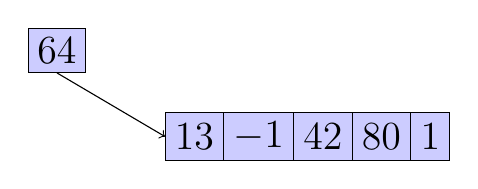
\begin{tikzpicture}[queue/.style = {fill = blue!20, font = \sffamily\Large\bfseries, rectangle split, rectangle split parts = 5, rectangle split horizontal, draw, anchor = center}, new/.style = {fill = blue!20, font = \sffamily\Large\bfseries, rectangle, draw, anchor = center}]
   \node [queue] (queue)  {$13$\nodepart{two}$-1$
   \nodepart{three}$42$\nodepart{four}$80$\nodepart{five}$1$};
   \node [new, above left = 0.5cm and 1cm of queue] (n) {$64$};
   \draw [->] (n.south) -- (queue.west);
\end{tikzpicture}

% file : exemple suppression

\vspace{3cm}
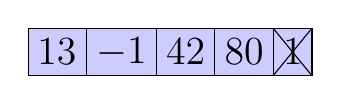
\begin{tikzpicture}[queue/.style = {fill = blue!20, font = \sffamily\Large\bfseries, rectangle split, rectangle split parts = 5, rectangle split horizontal, draw, anchor = center}]
   \node [queue] (queue)  {$13$\nodepart{two}$-1$
   \nodepart{three}$42$\nodepart{four}$80$\nodepart{five}$1$};
   \draw (1.8,0.3) -- (1.31,-0.3);
   \draw (1.8,-0.3) -- (1.31,0.3);
\end{tikzpicture}

\end{document}
